\documentclass{article}

\usepackage{amsmath}
\usepackage{amsfonts}
\usepackage{commath}
\usepackage[margin=1in]{geometry}
\usepackage{xfrac}
\usepackage{tkz-euclide}

\title{PHY202 Portfolio 3}
\author{Nicolas Nytko}
\date{November 18, 2016}

\nonumber

\begin{document}
\maketitle
\newpage
\section{Lenz's Law}
\subsection{Magnetic Flux}
The amount of electric field passing through an area can be calculated by the equation for magnetic flux.
\[ \Phi_B = \int \vec{B} \cdot d\vec{A} \]
The area must be an open surface in 3D.  If it is closed then there will be net magnetic field of 0.
\subsubsection{Problem Solving}
To calculate magnetic flux, first identify the magnetic field and the area you are getting flux in.  In most cases, $\vec{B}$ will be constant with respect to area so it can be pulled out of the integral.
\[ \Phi_B = \vec{B} \cdot \int d\vec{A} \]
Identify which direction the area is pointing in.  If a direction is not explicitly given, assume it points along a positive axis.  Integrate $d\vec{A}$, which in most cases $\int d\vec{A} = A$, so just find the area of the surface.
\[ \Phi_B = \vec{B} \cdot \vec{A} \]
\[ \Phi_B = \norm{\vec{B}} \norm{\vec{A}} \cos \theta \]
At this point, plug in the given values of $B$ and $A$ and solve for flux.
\subsection{Lenz's Law}
In 1834, Russian physicist Heinrich Lenz said:
\begin{quote}
{The direction of current induced in a conductor by a changing magnetic field due to Faraday's law of induction will be such that it will create a field that opposes the change that produced it.}
\end{quote}
This is shown as the negative sign in Faraday's Law:
\[ \varepsilon = -\frac{\partial \Phi}{\partial t} \]
In problem solving, the current will always be opposite of the direction of the flux derivative.
\section{Faraday's Law}
Faraday's law of induction states that the induced electromotive force in a closed circuit is equal to the negative rate of change of the magnetic flux enclosed in the circuit.
\[ \varepsilon = -N\frac{d\Phi_B}{dt} \]
Where N is the total number of loops in the circuit, $d\Phi_B$ is the change in flux, and $dt$ is the change in time.  This can be simplified into the equation:
\[ \abs{\varepsilon} = Blv \]
Where $B$ is the magnitude of the magnetic field, $l$ is the length of the object in the magnetic field, and $v$ is the velocity of the object going into the field.
To find the generated EMF in an AC generator, the following equation is used:
\[ \varepsilon = NBA\omega\sin(\omega t) \]
$\omega$ is the angular frequency in radians per second of the generator.
\subsection{Self-Inductance}
An inductor can create opposite EMF when it is faced with a change in EMF.  This is given by the equation:
\[ \varepsilon = -L\frac{dI}{dt} \]
Where $L$ is the value of self-inductance, $dI$ is the change in current and $dt$ is the change in time.  To calculate the self-inductance of an inductor, the following two formulas can be used:
\[ L = \frac{N\Phi_B}{I} \]
\[ L = \frac{\mu_0N^2A}{l} \]
$N$ is the total number of loops in the circuit, $I$ is the current flowing through the circuit, $\Phi_B$ is the magnetic flux.
For the second equation, $A$ is the cross-sectional area and $l$ is the length.
\section{LR and LC Circuits}
\subsection{LR Circuits}
In an LR Circuit, the equation for an energizing inductor is given as:
\[ I = \frac{\epsilon}{R}\left( 1 - e^{-\sfrac{t}{\tau}} \right)\]
$\frac{\epsilon}{R}$ is the current in the circuit. $\tau$ is the LR time constant, it is equal to $\frac{L}{R}$.
The equation for a de-energizing inductor is
\[ I = \frac{\epsilon}{R}e^{-\sfrac{t}{\tau}} \]
To find the potential energy of an inductor, use:
\[ U = \frac{1}{2} LI^2 \]
Where $L$ is the value of inductance and $I$ is the current.
\subsubsection{Problem Solving with a Switch}
When an LR circuit has a switch that has been closed for a long time, the inductor will act as a wire because there is no change in current.  When the switch is just closed, there will be no current because the inductor is opposing all of the change.

When an LR circuit has a switch that has just been open, the current will not change.  If the switch has been open for a long time there will be no current because any source of potential will be cut off.

For any time between that, you will have to use the energizing or de-energizing inductor formulas with the values of $t$.  Find the value of $\tau$ using $\tau=\sfrac{L}{R}$.
\subsection{LC Circuits}
When an inductor and capacitor are in series in a circuit, the current will ``bounce'' between them and create an alternating current.  The charge is described as a cosine wave, where the capacitor will first be filled at full charge.
\[Q(t)=Q_{max}\cos(\omega t)\]
The current is 90 degrees ahead of the charge.
\[I(t) = -I_{max}\sin(\omega t) \]
\[I(t) = -\omega Q_{max}(\omega t)\]
To find the angular speed in radians per second, $\omega_0$ use the following equation
\[\omega_0 = \frac{1}{\sqrt{LC}}\]
Where $L$ is the inductance of the circuit and $C$ is the capacitance of the circuit. To get the frequency in hertz, divide by $2\pi$.
\[\omega=2\pi f\]
\[f = \frac{\omega}{2\pi}\]
\section{Driven RLC Circuits}
In an RLC circuit, the charge is given by the following sinusoidal formula:
\[Q(t)=Q_{max}e^{-\sfrac{Rt}{2L}}\cos\left(\omega_dt\right)\]
To find $\omega_d$, the angular speed of a driven RLC circuit:
\[\omega_d=\left[ \frac{1}{LC} - \left(\frac{R}{2L}\right)^2 \right]^\frac{1}{2}\]
\subsection{Average Voltage}
Since the average of a sine wave is zero, to find the average voltage something called the \textit{root-mean-square} is used.  To find $V_{RMS}$, divide the voltage by $\sqrt{2}$.
\[V_{RMS}=\frac{V}{\sqrt{2}}\]
\subsection{Reactance}
Reactance in an inductor and capacitor is analogous to the resistor of a circuit. To find the reactance of an inductor:
\[X_L = 2\pi fL = \omega L\]
To find the reactance of a capacitor:
\[X_C = \frac{1}{2\pi fC} = \frac{1}{\omega C}\]
The impedance of a circuit is the effective resistance in an AC circuit, which is combined from the two reactances and the resistance, units in ohms.
\[Z=\sqrt{R^2+\left(X_L-X_C\right)^2}\]
\subsection{Phase Angle}
The phase angle is the angle that the voltage leads the current by.  It is calculated by:
\[ \tan\phi = \frac{X_L - X_C}{R} \]
\subsection{Drawing Phasors}
A phasor diagram represents voltage or current across a cdevice in an AC circuit.  It is a graph that rotates at angular speed $\omega$.  The projection of the vector onto the y-axis gives the magnitude at that point in time.
\subsubsection{Reactance Phasors}
To draw a reactance phasor diagram, draw $X_L$ along the positive Y axis, draw $X_C$ along the negative Y axis, and draw the resistance, $R$, along the positive X axis. Then, perform vector addition to get the impedance.
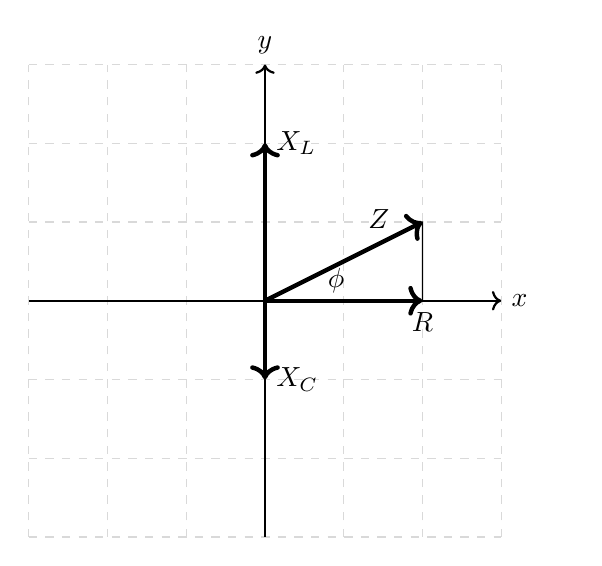
\begin{tikzpicture}
  \coordinate (A) at (0,0);
  \coordinate (B) at (2,0);
  \coordinate (C) at (2,1);
  \draw[help lines, color=gray!30, dashed] (-3,-3) grid (3,3);
\draw[->,thick] (-3,0)--(3,0) node[right]{$x$};
\draw[->,thick] (0,-3)--(0,3) node[above]{$y$};
\draw (A)--(B)--(C)--cycle;
\draw[->,ultra thick] (0,0)--(0,2) node[right]{$X_L$};
\draw[->,ultra thick] (0,0)--(0,-1) node[right]{$X_C$};
\draw[->,ultra thick] (0,0)--(2,0) node[below]{$R$};
\draw[->,ultra thick] (0,0)--(2,1);
\tkzLabelSegment[above left=12pt](B,C){$Z$};
\node[text width=3cm] at (2.3,0.25) {$\phi$};
\end{tikzpicture} \\
In this case, $\phi$ is the angle that the impedance leads the resistance.
\subsubsection{Voltage Phasors}
To draw a voltage phasor diagram, draw $V_L$ along the positive Y axis, draw $V_C$ along the negative Y axis, and draw $V_R$, along the positive X axis. Then, perform vector addition to get the voltage of the circuit.
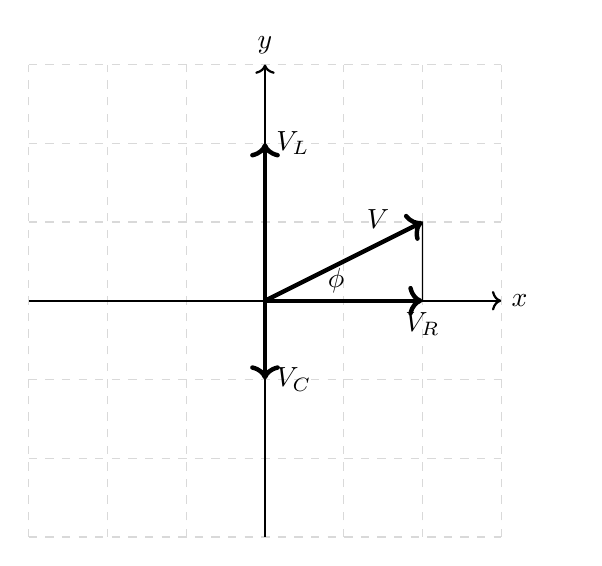
\begin{tikzpicture}
  \coordinate (A) at (0,0);
  \coordinate (B) at (2,0);
  \coordinate (C) at (2,1);
  \draw[help lines, color=gray!30, dashed] (-3,-3) grid (3,3);
\draw[->,thick] (-3,0)--(3,0) node[right]{$x$};
\draw[->,thick] (0,-3)--(0,3) node[above]{$y$};
\draw (A)--(B)--(C)--cycle;
\draw[->,ultra thick] (0,0)--(0,2) node[right]{$V_L$};
\draw[->,ultra thick] (0,0)--(0,-1) node[right]{$V_C$};
\draw[->,ultra thick] (0,0)--(2,0) node[below]{$V_R$};
\draw[->,ultra thick] (0,0)--(2,1);
\tkzLabelSegment[above left=12pt](B,C){$V$};
\node[text width=3cm] at (2.3,0.25) {$\phi$};
\end{tikzpicture} \\
In this case, $\phi$ is the angle that the voltage leads the current.
\subsubsection{ELI the ICE man}
A mnemonic to remember the sign of the phase angle in an inductor or capacitor is \textit{ELI the ICE man}.  $\varepsilon$ leads $I$ in an inductor ($L$),  $I$ leads $\varepsilon$ in a capacitor ($C$).
\section{EM Waves}
Maxwell stated that changing electromagnetic fields should produce changing magnetic fields and vice-versa.  The equations for $\vec{E}$ field and $\vec{B}$ field in a wave are:
\[\vec{E} = E\sin(kx - \omega t)\hat{\jmath}\]
\[\vec{B} = B\sin(kx - \omega t)\hat{k}\]
The wave number, $k$ is equal to $2\pi$ divided by the wavelength.  It is the number of cycles/radians per unit distance.
\[k=\frac{2\pi}{\lambda}\]
The ratio of the electric field to the magnetic field is equal to the speed of light.
\[c = \frac{1}{\sqrt{\mu_0\epsilon_0}}=\frac{E}{B}=\lambda f\]
The intensity and direction of an EM wave can be found by calculating the \textit{Poynting} vector, $\vec{S}$.
\[\vec{S}=\frac{\vec{E} \times \vec{B}}{\mu_0}\]
To find just the intensity of an EM wave, this simplified formula can be used:
\[ I = \frac{EB}{2\mu_0} \]
The direction of the Poynting vector determines the direction of the propagating wave, while the magnitude determines the average intensity of the wave.
\end{document}